\newpage
\subsection{Excluding certain projects from the export}

You may find it sometimes necessary to exclude certain projects from your diagram export (such as the \texttt{MocaTree} model used in Part V).
Some reasons for this could be (i) because the project is still a work in progress and simply not ready to be exported, (ii) because the
complete project is present in the Eclipse workspace but has not been modelled completely in EA, and you wish to do this gradually on-demand, (iii) because the
project is not meant to be present in your Eclipse workspace as generated code and is instead provided via a plugin (this is usually the case for standard
metamodels like Ecore, UML etc.), or (iv) because the project is rather large and stable and you do not want to wait for EA to process a known, unchanging
model. Whatever the reason, you can prevent unnecessary exports by setting a certain \emph{tagged value} of the project.

\begin{stepbystep}

\item Open your project in EA, and navigate to ``View/Tagged Values'' from the menu bar (\Cref{ea:view/Taggedvalues}).

\begin{figure}[htbp]
\begin{center}  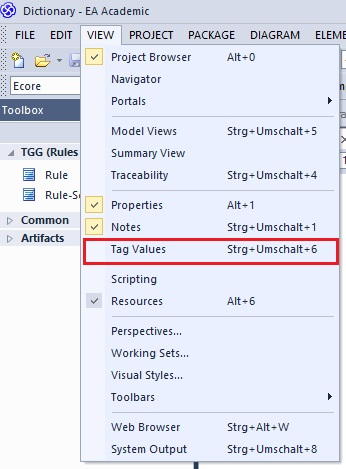
\includegraphics[width=0.5\textwidth]{ea_viewTaggedValues}
  \caption{Opening the tagged values view}  
  \label{ea:view/Taggedvalues}
\end{center}
\end{figure} 

\item The tagged value, \emph{Moflon::Export}, should already be present and be set to a default \texttt{true} value
(\Cref{ea:moflonExportTG}). If you want the project to be ignored by the eMoflon's validation and/or export functions, change the value to
\texttt{false} (and conversely back to \texttt{true} to export it again).

\begin{figure}[htbp]
\begin{center}
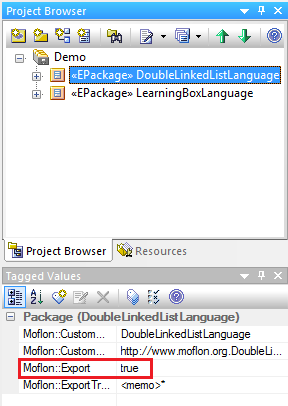
\includegraphics[width=0.5\textwidth]{ea_moflonExportTG}
  \caption{The \texttt{Moflon::Export} setting determines ignored projects}  
  \label{ea:moflonExportTG}
\end{center}
\end{figure}

\end{stepbystep}
